% This is text associated with the open textbook "Open Electromagnetics"
% See immediately below for author, date
% This work is licensed under the Creative Commons Attribution-ShareAlike 4.0 International License. (CC BY-SA 4.0) 
% To view a copy of the license, visit http://creativecommons.org/licenses/by-sa/4.0/

%ORB TITLE Angles of Reflection and Refraction
%ORB AUTHOR 0        # S.W. Ellingson, Virginia Tech (ellingson@vt.edu)
%ORB DATE 20191119   # yyyymmdd
%ORB ABSTRACT 

\label{m0168_Angles_of_Reflection_and_Refraction} % <-- Must match name of this file and module directory name.  Don't mess with this!
%\index{impedance!wire|(}

Consider the situation shown in Figure~\ref{m0168_fOblique}: 
%
\begin{figure}[b!]
\begin{center}
\pdftooltip{{  % note double braces
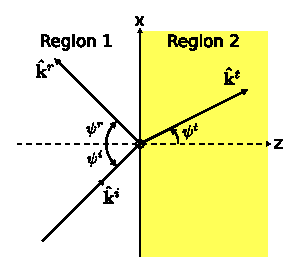
\includegraphics[width=0.8\columnwidth]{modules/m0168_fOblique.eps} 
% https://commons.wikimedia.org/wiki/File:Upw_incident_obliquely_on_planar_boundary.svg
}}{Incident wave in direction small k hat superscript i at angle small psi superscript i from negative z. Transmitted wave small k hat superscript t at angle small psi superscript t to positive z. Reflected wave small k hat superscript r at an angle small psi superscript r to negative z.}
\end{center}
\centerline{\scriptsize 
\copyright~\hyperref[m0168_fOblique_Credit]{C.\ Wang} 
\href{https://creativecommons.org/licenses/by-sa/4.0/}{CC BY-SA 4.0} 
} 
\caption{
\label{m0168_fOblique}
A uniform plane wave obliquely incident on the planar boundary between two semi-infinite material regions.
}
\end{figure}
%
A uniform plane wave obliquely incident on the planar boundary between two semi-infinite material regions.
Let a point on the boundary be represented as the position vector
%
\begin{equation}
{\bf r}_0 = \hat{\bf x}x + \hat{\bf y}y
\end{equation}
%
In both Sections~\ref{m0167_Oblique_Incidence_TE} (``Plane Waves at Oblique Incidence on a Planar Boundary: TE Case'') and 
\ref{m0164_Oblique_Incidence_TM} 
(``Plane Waves at Oblique Incidence on a Planar Boundary: TM Case''), it is found that 
%
\begin{equation}
{\bf k}^i\cdot{\bf r}_0 = {\bf k}^r\cdot{\bf r}_0 = {\bf k}^t\cdot{\bf r}_0
\label{m0168_eSL}
\end{equation}
%
In this expression, 
%
\begin{flalign}
{\bf k}^i &= \beta_1 \hat{\bf k}^i \\
{\bf k}^r &= \beta_1 \hat{\bf k}^r \\
{\bf k}^t &= \beta_2 \hat{\bf k}^t 
\end{flalign}
%
where $\hat{\bf k}^i$, $\hat{\bf k}^r$, and $\hat{\bf k}^t$ are unit vectors in the direction of incidence, reflection, and transmission, respectively; and
$\beta_1$ and $\beta_2$ are the phase propagation constants in Region~1 (from which the wave is incident) and Region~2, respectively.  
Equation~\ref{m0168_eSL} is essentially a boundary condition that enforces continuity of the phase of the electric and magnetic fields across the boundary, and is sometimes referred to as the ``phase matching'' requirement.
Since the same requirement emerges independently in the TE and TM cases, and since any plane wave may be decomposed into TE and TM components, the requirement must apply to any incident plane wave regardless of polarization.

Equation~\ref{m0168_eSL} is the key to finding the direction of reflection $\psi^r$ and direction of transmission $\psi^t$.
First, observe:
%
\begin{flalign}
\hat{\bf k}^i &= \hat{\bf x}\sin\psi^i + \hat{\bf z}\cos\psi^i  \\
\hat{\bf k}^r &= \hat{\bf x}\sin\psi^r - \hat{\bf z}\cos\psi^r \\
\hat{\bf k}^t &= \hat{\bf x}\sin\psi^t + \hat{\bf z}\cos\psi^t 
\end{flalign}
%
Therefore, we may express Equation~\ref{m0168_eSL} in the following form
%
\begin{flalign}
 \beta_1\left(\hat{\bf x}\sin\psi^i + \hat{\bf z}\cos\psi^i\right)\cdot\left(\hat{\bf x}x + \hat{\bf y}y\right) \nonumber \\
=\beta_1\left(\hat{\bf x}\sin\psi^r - \hat{\bf z}\cos\psi^r\right)\cdot\left(\hat{\bf x}x + \hat{\bf y}y\right) \nonumber \\
=\beta_2\left(\hat{\bf x}\sin\psi^t + \hat{\bf z}\cos\psi^t\right)\cdot\left(\hat{\bf x}x + \hat{\bf y}y\right) 
\end{flalign}
%
which reduces to
%
\begin{equation}
\beta_1 \sin\psi^i =\beta_1 \sin\psi^r =\beta_2 \sin\psi^t 
\label{m0168_eA3}
\end{equation}
%
Examining the first and second terms of Equation~\ref{m0168_eA3}, and noting that $\psi^i$ and $\psi^r$ are both limited to the range $-\pi/2$ to $+\pi/2$, we find that:
%
\begin{equation}
\boxed{ \psi^r = \psi^i }
\end{equation}
%
In plain English:  
%
%%%%%%%%%%%%%%%%%%%%%%%%%%%%%%%%%%%%%%%%%%%%%%%
%ORB HIGHLIGHT
\begin{mdframed}[backgroundcolor=yellow!20,nobreak=true] 
Angle of reflection equals angle of incidence.
\end{mdframed}
%%%%%%%%%%%%%%%%%%%%%%%%%%%%%%%%%%%%%%%%%%%%%%%
%
Examining the first and third terms of Equation~\ref{m0168_eA3}, we find that
%
\begin{equation}
\beta_1 \sin\psi^i = \beta_2 \sin\psi^t 
\label{m0168_eASL}
\end{equation}
%
Since 
$\beta_1=\omega\sqrt{\mu_1\epsilon_1}$ and 
$\beta_2=\omega\sqrt{\mu_2\epsilon_2}$, Equation~\ref{m0168_eASL} expressed explicitly in terms of the constitutive parameters is:
%
\begin{equation}
\sqrt{\mu_1\epsilon_1} \sin\psi^i = \sqrt{\mu_2\epsilon_2} \sin\psi^t
\label{m0168_eAt2}
\end{equation}
%
Thus, we see that $\psi^t$ does not depend on frequency, except to the extent that the constitutive parameters might.
We may also express this relationship in terms of the \emph{relative} values of constitutive parameters; i.e.,
$\mu_1=\mu_{r1}\mu_0$, 
$\epsilon_1=\epsilon_{r1}\epsilon_0$, 
$\mu_2=\mu_{r2}\mu_0$, and
$\epsilon_2=\epsilon_{r2}\epsilon_0$.
In terms of the relative parameters:
%
\begin{equation}
\boxed{ \sqrt{\mu_{r1}\epsilon_{r1}} \sin\psi^i = \sqrt{\mu_{r2}\epsilon_{r2}} \sin\psi^t }
\label{m0168_eAt3}
\end{equation}
%
This is known as \emph{Snell's law}
\index{Snell's law}
or the \emph{law of refraction}.
Refraction
\index{refraction}
is simply transmission with the result that the direction of propagation is changed.
%
%%%%%%%%%%%%%%%%%%%%%%%%%%%%%%%%%%%%%%%%%%%%%%%
%ORB HIGHLIGHT
\begin{mdframed}[backgroundcolor=yellow!20,nobreak=true] 
Snell's law (Equation~\ref{m0168_eAt3}) determines the angle of refraction (transmission).
\end{mdframed}
%%%%%%%%%%%%%%%%%%%%%%%%%%%%%%%%%%%%%%%%%%%%%%%
%
The associated formula for $\psi^t$ explicitly is:
%
\begin{equation}
\psi^t = \arcsin\left(\sqrt{\frac{\mu_{r1}\epsilon_{r1}}{\mu_{r2}\epsilon_{r2}}} \sin\psi^i \right)  
\label{m0168_eAt}
\end{equation}
%
For the common special case of non-magnetic media, one assumes $\mu_{r1}=\mu_{r2}= 1$. 
In this case, Snell's law simplifies to:
%
\begin{equation}
\sqrt{\epsilon_{r1}} \sin\psi^i = \sqrt{\epsilon_{r2}} \sin\psi^t
\label{m0168_eAtnm}
\end{equation}
%
In optics, it is common to express permittivities in terms of indices of refraction; 
\index{index of refraction}
e.g., 
$n_1\triangleq\sqrt{\epsilon_{r1}}$ and
$n_2\triangleq\sqrt{\epsilon_{r2}}$.
Thus, Snell's law in optics is often expressed as:
%
\begin{equation}
n_1 \sin\psi^i = n_2 \sin\psi^t
\label{m0168_eAtnmo}
\end{equation}

When both media are non-magnetic, Equation~\ref{m0168_eAt} simplifies to
%
\begin{equation}
\psi^t = \arcsin\left(\sqrt{\frac{\epsilon_{r1}}{\epsilon_{r2}}} \sin\psi^i \right)  
\label{m0168_eAt2}
\end{equation}
%
When $\epsilon_{r2}>\epsilon_{r1}$, we observe that $\psi^t < \psi^i$.  
In other words, the transmitted wave travels in a direction that is closer to the surface normal than the angle of incidence. 
This scenario is demonstrated in the following example.

%%%%%%%%%%%%%%%%%%%%%%%%%%%%%%%%%%%%%%%%%%%%%%%
%ORB EXAMPLE
~\\ \begin{example} 
\begin{mdframed}[backgroundcolor=brown!20,linecolor=brown!20]\raggedright
Refraction of light at an air-glass boundary.
\\~\\
Figure~\ref{m0168_fFenytores} shows a narrow beam of light that is incident from air to glass at an angle $\psi^i=60^{\circ}$.
As expected, the angle of reflection $\psi^r$ is observed to be equal to $\psi^i$.
The angle of refraction $\psi^t$ is observed to be $35^{\circ}$.
What is the relative permittivity of the glass?\\
~\\

{\bf Solution.} 
Since the permittivity of glass is greater than that of air, we observe the expected result $\psi^t<\psi^i$.
Since glass is non-magnetic, the expected relationship between these angles is given by Equation~\ref{m0168_eAtnm}.
Solving that equation for the relative permittivity of the glass, we obtain:
%
\begin{equation}
\epsilon_{r2} = \epsilon_{r1} \left(\frac{\sin\psi^i}{\sin\psi^t}\right)^2 \cong \underline{2.28} 
\end{equation}
%
\end{mdframed}
% note figures will need to go between "\end{mdframed}" and "\end{example}"
%
\begin{figure}
\begin{center}
\pdftooltip{{  % note double braces
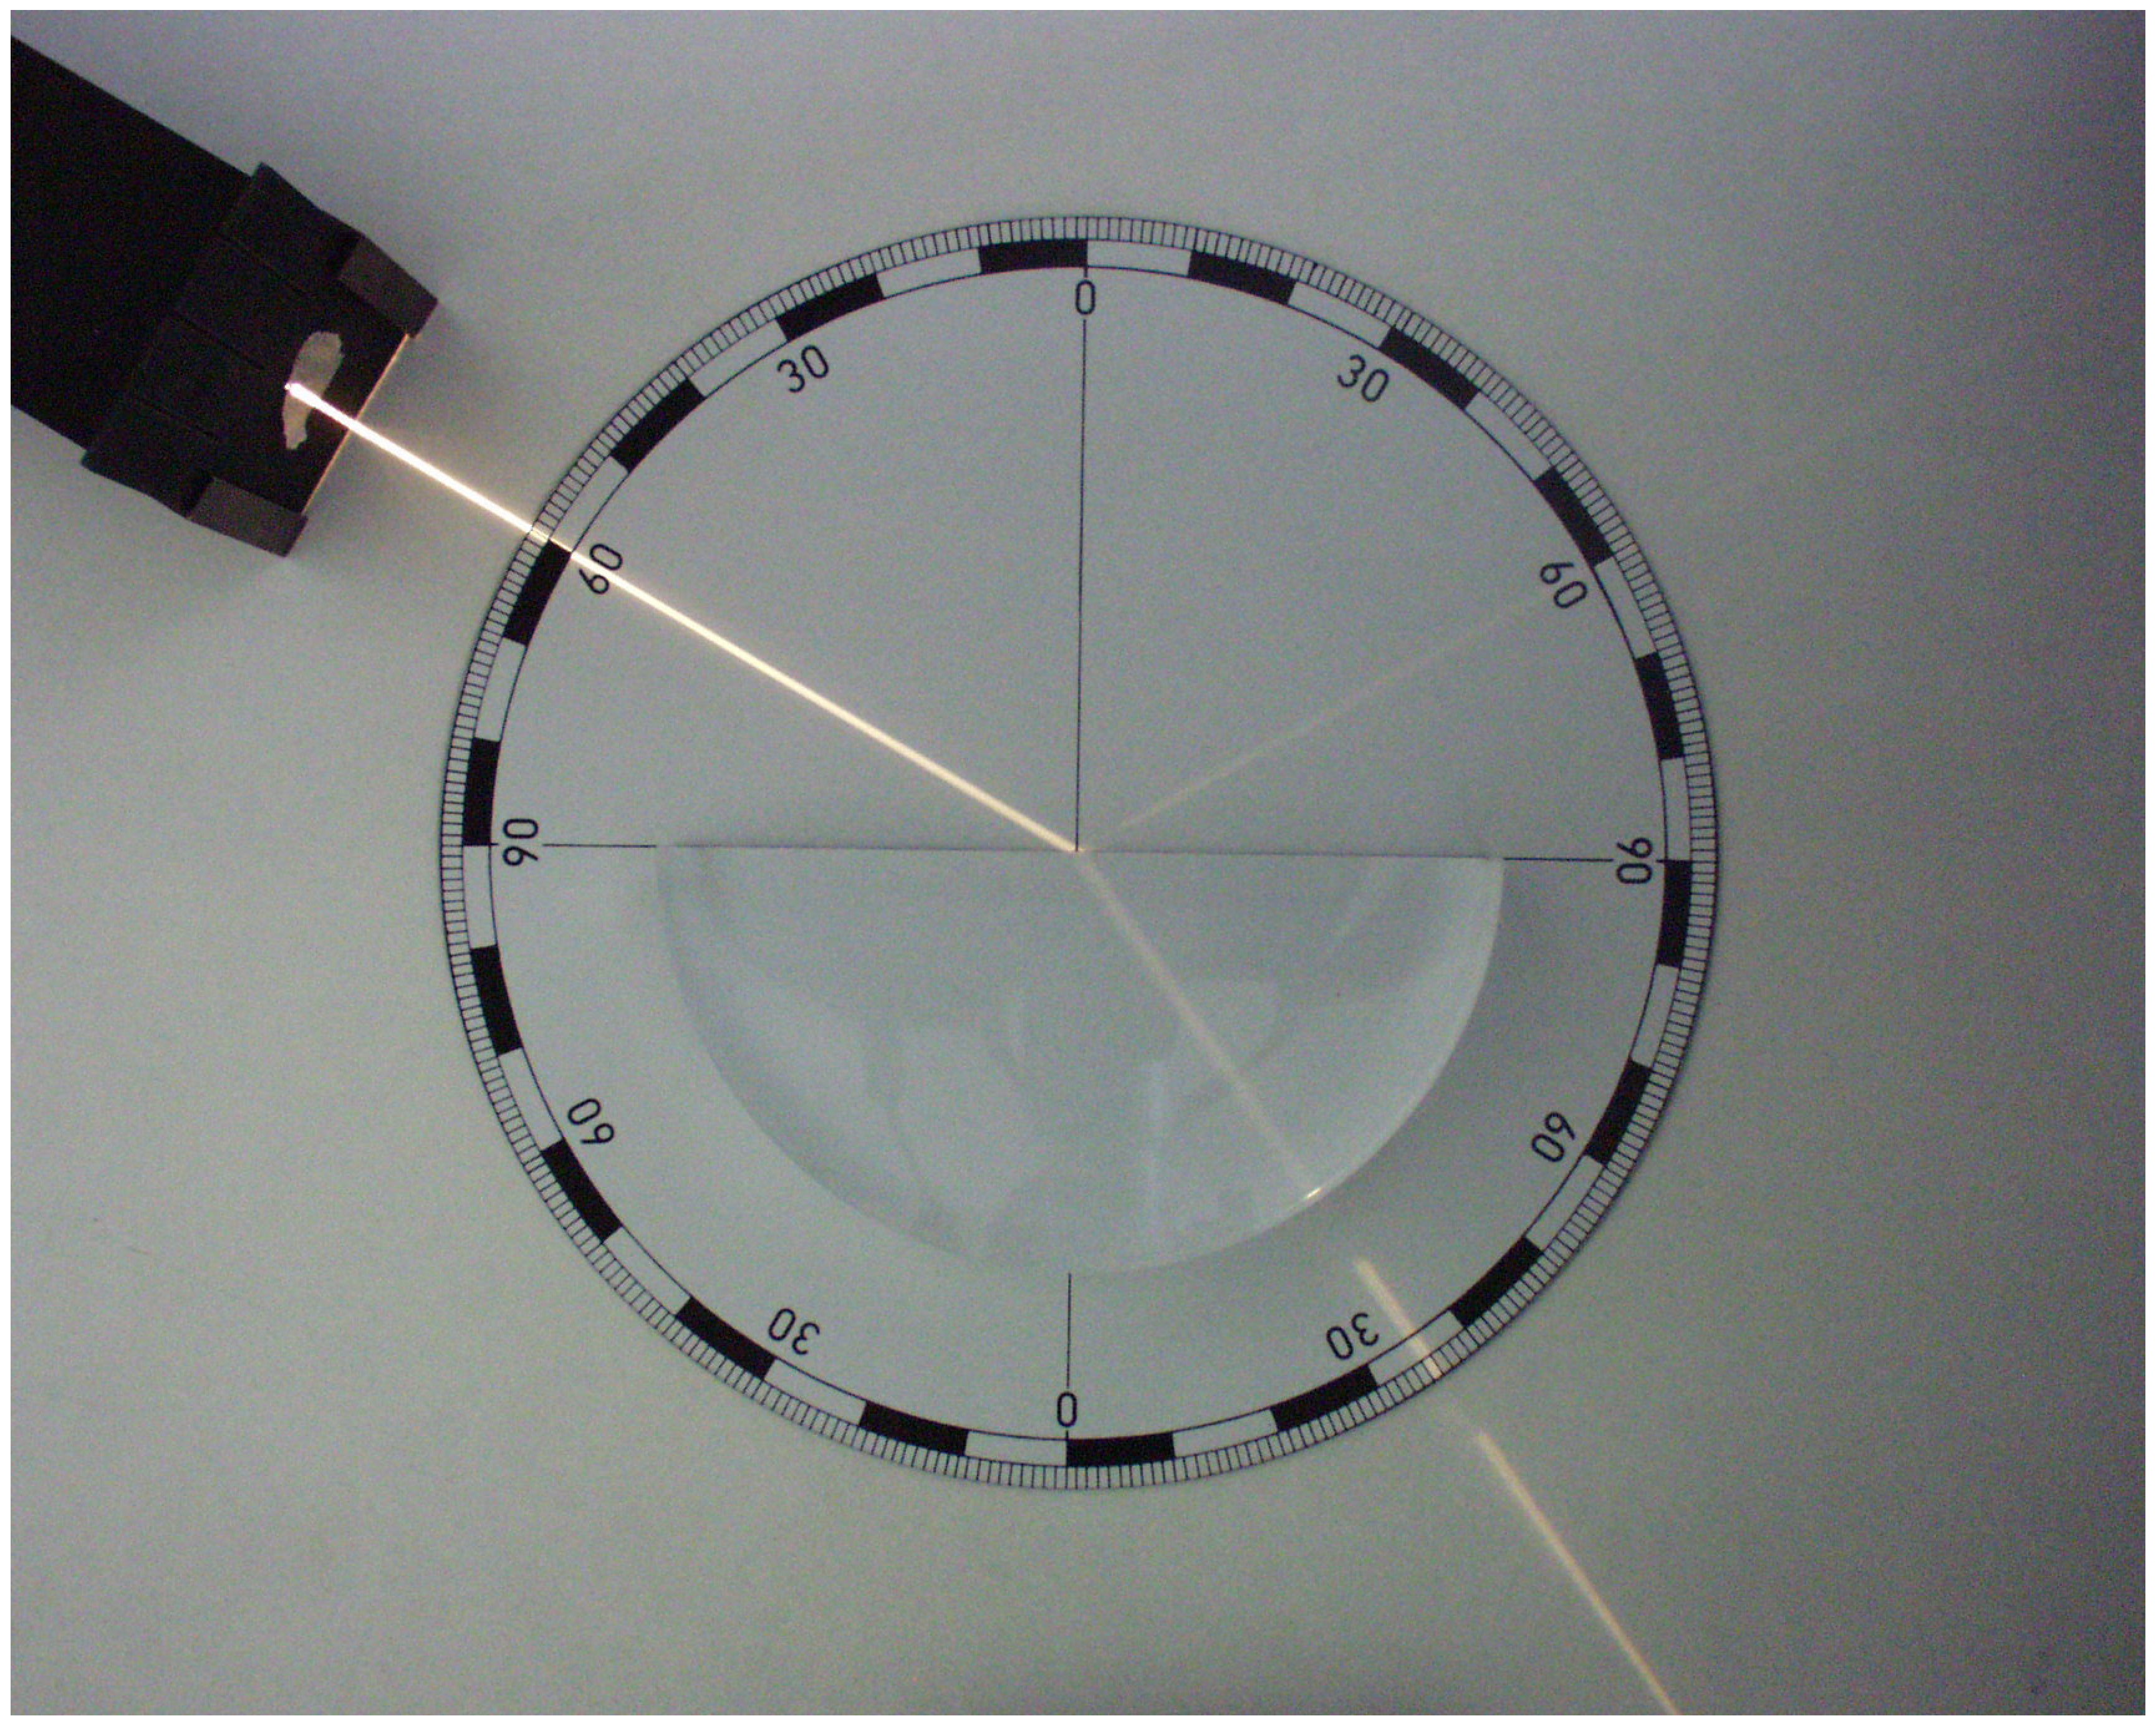
\includegraphics[width=\columnwidth]{modules/m0168_fFenytores.eps} 
% https://commons.wikimedia.org/wiki/File:F%C3%A9nyt%C3%B6r%C3%A9s.jpg
}}{Laser reflects through center of the flat edge of semicircular glass and comes out at an angle of 35 degrees southeast.}
\end{center}
\centerline{\scriptsize 
\copyright~\hyperref[m0168_fFenytores_Credit]{Z.\ S\'{a}ndor } 
\href{https://creativecommons.org/licenses/by-sa/3.0/}{CC BY-SA 3.0} 
} 
\caption{
\label{m0168_fFenytores}
Angles of reflection and refraction for a light wave incident from air onto glass.
}
\end{figure}
%
\end{example}
%%%%%%%%%%%%%%%%%%%%%%%%%%%%%%%%%%%%%%%%%%%%%%%

When a wave travels in the reverse direction -- i.e., from a non-magnetic medium of higher permittivity to a medium of lower permittivity -- one finds $\psi^t>\psi^r$.
In other words, the refraction is \emph{away} from the surface normal. 
Figure~\ref{m0168_fObliqueIntoWater} shows an example from common experience.
%
\begin{figure}
\begin{center}
\pdftooltip{{  % note double braces
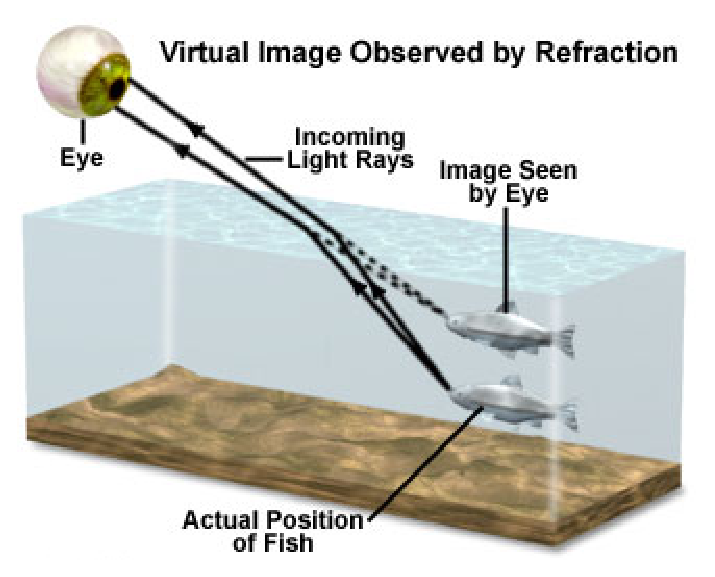
\includegraphics[width=0.8\columnwidth]{modules/m0168_fRefractionn.eps} 
% https://kids.kiddle.co/Image:Refractionn.jpg
}}{An eyeball (top left) looking at two fish in water (bottom right). Light rays enter the eyes. First ray shows actual position of the fish is lower than the second image seen by the eye.}
\end{center}
\centerline{\scriptsize 
\copyright~\hyperref[m0168_fObliqueIntoWater_Credit]{G.\ Saini} 
\href{https://creativecommons.org/licenses/by-sa/4.0/}{CC BY-SA 4.0} 
} 
\caption{
\label{m0168_fObliqueIntoWater}
Refraction accounts for the apparent displacement of an underwater object from the perspective of an observer above the water.
}
\end{figure}

%%%%%%%%%%%%%%%%%%%%%%%%%%%%%%%%%%%%%%%%%%%%%%%
%ORB HIGHLIGHT
\begin{mdframed}[backgroundcolor=yellow!20,nobreak=true] 
In non-magnetic media, when
$\epsilon_{r1}<\epsilon_{r2}$, $\psi_t<\psi_i$ (refraction toward the surface normal).
When 
$\epsilon_{r1}>\epsilon_{r2}$, $\psi_t>\psi_i$ (refraction away from the surface normal).
\end{mdframed}
%%%%%%%%%%%%%%%%%%%%%%%%%%%%%%%%%%%%%%%%%%%%%%%

Under certain conditions, the $\epsilon_{r2}<\epsilon_{r1}$ case leads to the following surprising observation:
When calculating $\psi^t$ using, for example, Equation~\ref{m0168_eAt}, one finds that   
$\sqrt{\epsilon_{r1}/\epsilon_{r2}} \sin\psi^i$ can be greater than 1.
Since the $\sin$ function yields values between $-1$ and $+1$, the result of the $\arcsin$ function is undefined.
This odd situation is addressed in Section~\ref{m0169_Total_Internal_Reflection}.
For now, we will simply note that this condition leads to the phenomenon of \emph{total internal reflection}.
\index{total internal reflection}
For now, all we can say is that when $\epsilon_{r2}<\epsilon_{r1}$, $\psi^t$ is able to reach $\pi/2$ radians, which corresponds to propagation parallel to the boundary. Beyond that threshold, we must account for the unique physical considerations associated with total internal reflection. 

We conclude this section with a description of the common waveguiding device known as the \emph{prism}, shown in Figure~\ref{m0168_Prism-side-fs_PNr-0117}.
\index{prism}
This particular device uses refraction to change the direction of light waves (similar devices can be used to manipulate radio waves as well).
%
\begin{figure}
\begin{center}
\pdftooltip{{  % note double braces
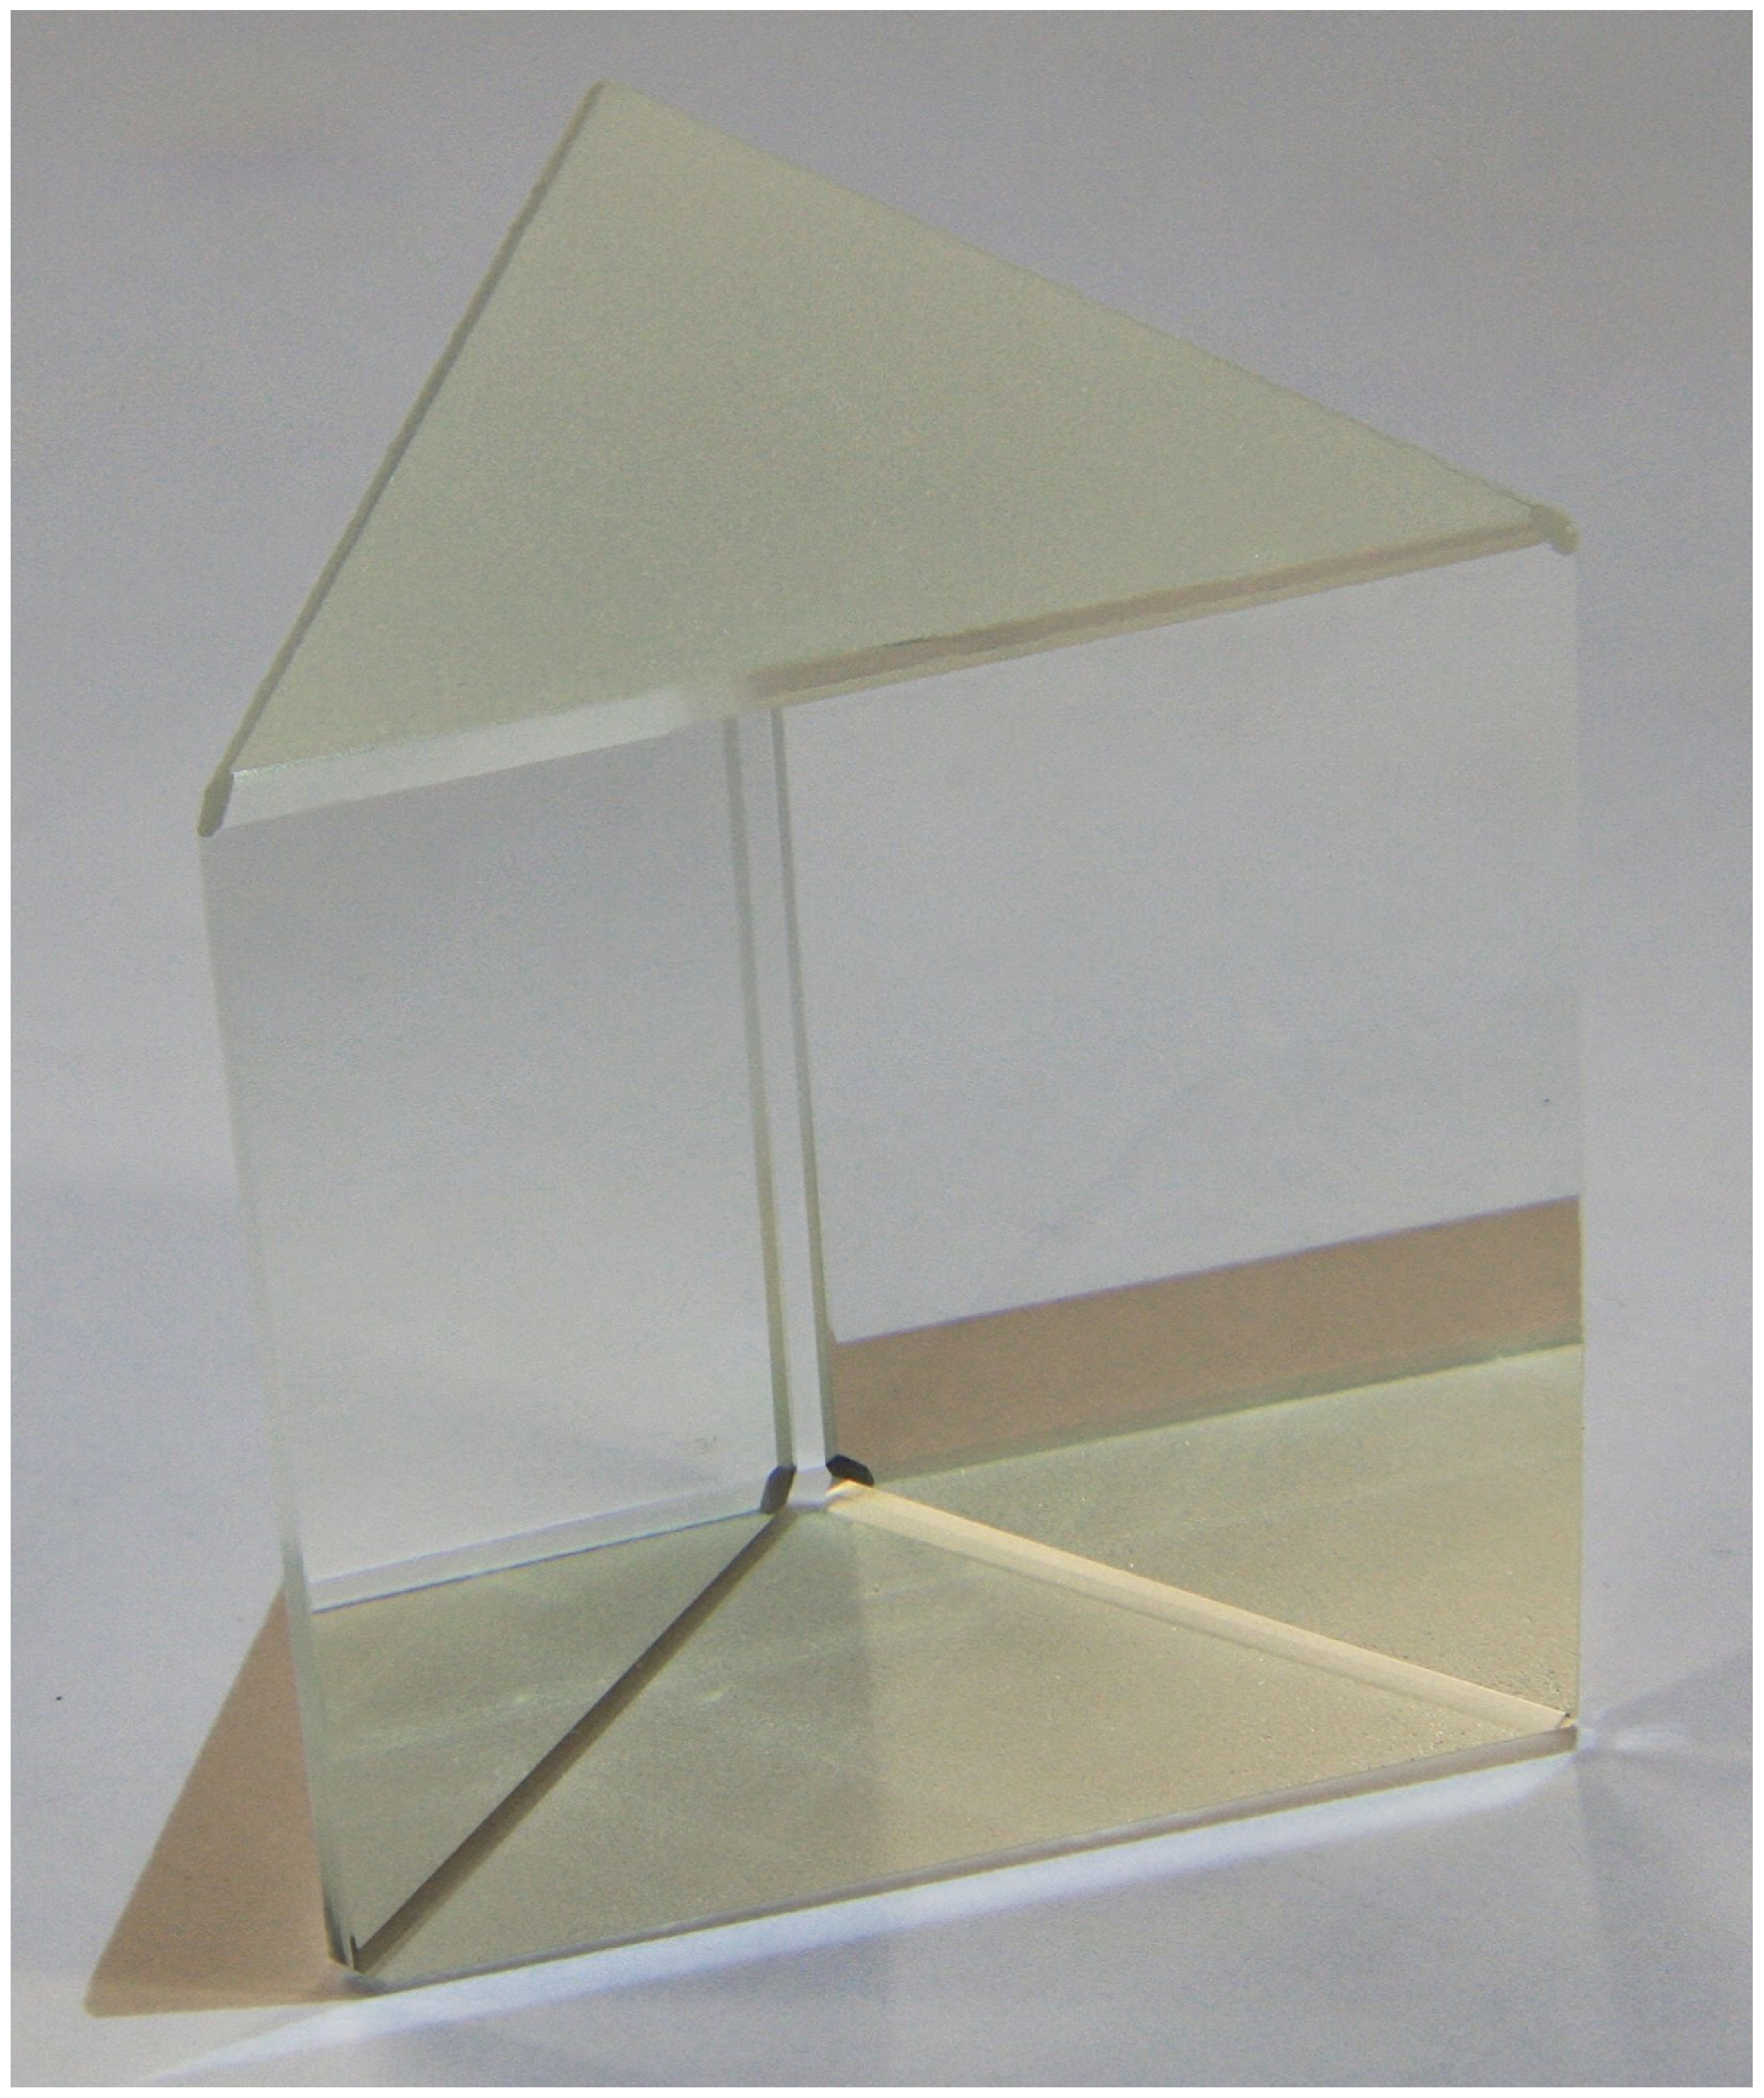
\includegraphics[width=0.8\columnwidth]{modules/m0168_Prism-side-fs_PNr-0117.eps} 
% https://commons.wikimedia.org/wiki/File:Prism-side-fs_PNr%C2%B00117.jpg
}}{A glass triangular prism.}
\end{center}
\centerline{\scriptsize 
\copyright~\hyperref[m0168_Prism-side-fs_PNr-0117_Credit]{D-Kuru} 
\href{https://creativecommons.org/licenses/by-sa/3.0/}{CC BY-SA 3.0} 
} 
\caption{
\label{m0168_Prism-side-fs_PNr-0117}
A typical triangular prism.
}
\end{figure}
%
Many readers are familiar with the use of prisms to separate white light into its constituent colors (frequencies), as shown in Figure~\ref{m0168_Prism_rainbow_schema}.
The separation of colors is due to frequency dependence of the material comprising the prism.
Specifically, the permittivity of the material is a function of frequency, and therefore the angle of refraction is a function of frequency.
Thus, each frequency is refracted by a different amount.
Conversely, a prism comprised of a material whose permittivity exhibits negligible variation with frequency will not separate incident white light into its constituent colors since each color will be refracted by the same amount.
%
\begin{figure}
\begin{center}
\pdftooltip{{  % note double braces
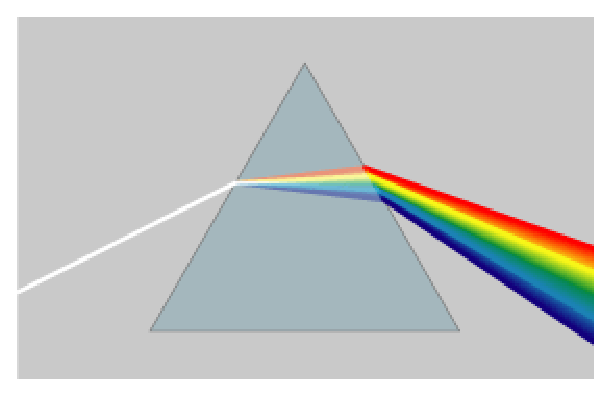
\includegraphics[width=0.8\columnwidth]{modules/m0168_Prism_rainbow_schema.eps} 
% https://commons.wikimedia.org/wiki/File:Prism-rainbow.svg (PNG: https://commons.wikimedia.org/wiki/File:Prism_rainbow_schema.png)
}}{A white ray of light entering a triangular prism from the left refracts through the triangle and into a rainbow as it travels to the right.}
\end{center}
\centerline{\scriptsize 
\copyright~\hyperref[m0168_Prism_rainbow_schema_Credit]{Suidroot} 
\href{https://creativecommons.org/licenses/by-sa/3.0/}{CC BY-SA 4.0} 
} 
\caption{
\label{m0168_Prism_rainbow_schema}
A color-separating prism.
}
\end{figure}

%%%%%%%%%%%%%%%%%%%%%

{\bf Additional Reading:}
\begin{itemize}
\item ``\href{https://en.wikipedia.org/wiki/Prism}{Prism}'' on Wikipedia.
\item ``\href{https://en.wikipedia.org/wiki/Refraction}{Refraction}'' on Wikipedia.
\item ``\href{https://en.wikipedia.org/wiki/Refractive_index}{Refractive index}'' on Wikipedia.
\item ``\href{https://en.wikipedia.org/wiki/Snell's_law}{Snell's law}'' on Wikipedia.
\item ``\href{https://en.wikipedia.org/wiki/Total_internal_reflection}{Total internal reflection}'' on Wikipedia.
\end{itemize}

% \index{impedance!wire|)}

% Other useful images:
% https://en.wikipedia.org/wiki/File:Pencil_in_a_bowl_of_water.svg

